\documentclass[a4paper,12pt,twoside]{memoir}

% Castellano
\usepackage[spanish,es-tabla]{babel}
\selectlanguage{spanish}
\usepackage[utf8]{inputenc}
\usepackage[T1]{fontenc}
\usepackage{lmodern} % Scalable font
\usepackage{microtype}
\usepackage{placeins}

\RequirePackage{booktabs}
\RequirePackage[table]{xcolor}
\RequirePackage{xtab}
\RequirePackage{multirow}

% Links
\usepackage[colorlinks]{hyperref}
\hypersetup{
	allcolors = {red}
}

% Ecuaciones
\usepackage{amsmath}

% Rutas de fichero / paquete
\newcommand{\ruta}[1]{{\sffamily #1}}

% Párrafos
\nonzeroparskip


% Imagenes
\usepackage{graphicx}
\newcommand{\imagen}[2]{
	\begin{figure}[!h]
		\centering
		\includegraphics[width=0.9\textwidth]{#1}
		\caption{#2}\label{fig:#1}
	\end{figure}
	\FloatBarrier
}

\newcommand{\imagenflotante}[2]{
	\begin{figure}%[!h]
		\centering
		\includegraphics[width=0.9\textwidth]{#1}
		\caption{#2}\label{fig:#1}
	\end{figure}
}



% El comando \figura nos permite insertar figuras comodamente, y utilizando
% siempre el mismo formato. Los parametros son:
% 1 -> Porcentaje del ancho de página que ocupará la figura (de 0 a 1)
% 2 --> Fichero de la imagen
% 3 --> Texto a pie de imagen
% 4 --> Etiqueta (label) para referencias
% 5 --> Opciones que queramos pasarle al \includegraphics
% 6 --> Opciones de posicionamiento a pasarle a \begin{figure}
\newcommand{\figuraConPosicion}[6]{%
  \setlength{\anchoFloat}{#1\textwidth}%
  \addtolength{\anchoFloat}{-4\fboxsep}%
  \setlength{\anchoFigura}{\anchoFloat}%
  \begin{figure}[#6]
    \begin{center}%
      \Ovalbox{%
        \begin{minipage}{\anchoFloat}%
          \begin{center}%
            \includegraphics[width=\anchoFigura,#5]{#2}%
            \caption{#3}%
            \label{#4}%
          \end{center}%
        \end{minipage}
      }%
    \end{center}%
  \end{figure}%
}

%
% Comando para incluir imágenes en formato apaisado (sin marco).
\newcommand{\figuraApaisadaSinMarco}[5]{%
  \begin{figure}%
    \begin{center}%
    \includegraphics[angle=90,height=#1\textheight,#5]{#2}%
    \caption{#3}%
    \label{#4}%
    \end{center}%
  \end{figure}%
}
% Para las tablas
\newcommand{\otoprule}{\midrule [\heavyrulewidth]}
%
% Nuevo comando para tablas pequeñas (menos de una página).
\newcommand{\tablaSmall}[5]{%
 \begin{table}
  \begin{center}
   \rowcolors {2}{gray!35}{}
   \begin{tabular}{#2}
    \toprule
    #4
    \otoprule
    #5
    \bottomrule
   \end{tabular}
   \caption{#1}
   \label{tabla:#3}
  \end{center}
 \end{table}
}

%
% Nuevo comando para tablas pequeñas (menos de una página).
\newcommand{\tablaSmallSinColores}[5]{%
 \begin{table}[H]
  \begin{center}
   \begin{tabular}{#2}
    \toprule
    #4
    \otoprule
    #5
    \bottomrule
   \end{tabular}
   \caption{#1}
   \label{tabla:#3}
  \end{center}
 \end{table}
}

\newcommand{\tablaApaisadaSmall}[5]{%
\begin{landscape}
  \begin{table}
   \begin{center}
    \rowcolors {2}{gray!35}{}
    \begin{tabular}{#2}
     \toprule
     #4
     \otoprule
     #5
     \bottomrule
    \end{tabular}
    \caption{#1}
    \label{tabla:#3}
   \end{center}
  \end{table}
\end{landscape}
}

%
% Nuevo comando para tablas grandes con cabecera y filas alternas coloreadas en gris.
\newcommand{\tabla}[6]{%
  \begin{center}
    \tablefirsthead{
      \toprule
      #5
      \otoprule
    }
    \tablehead{
      \multicolumn{#3}{l}{\small\sl continúa desde la página anterior}\\
      \toprule
      #5
      \otoprule
    }
    \tabletail{
      \hline
      \multicolumn{#3}{r}{\small\sl continúa en la página siguiente}\\
    }
    \tablelasttail{
      \hline
    }
    \bottomcaption{#1}
    \rowcolors {2}{gray!35}{}
    \begin{xtabular}{#2}
      #6
      \bottomrule
    \end{xtabular}
    \label{tabla:#4}
  \end{center}
}

%
% Nuevo comando para tablas grandes con cabecera.
\newcommand{\tablaSinColores}[6]{%
  \begin{center}
    \tablefirsthead{
      \toprule
      #5
      \otoprule
    }
    \tablehead{
      \multicolumn{#3}{l}{\small\sl continúa desde la página anterior}\\
      \toprule
      #5
      \otoprule
    }
    \tabletail{
      \hline
      \multicolumn{#3}{r}{\small\sl continúa en la página siguiente}\\
    }
    \tablelasttail{
      \hline
    }
    \bottomcaption{#1}
    \begin{xtabular}{#2}
      #6
      \bottomrule
    \end{xtabular}
    \label{tabla:#4}
  \end{center}
}

%
% Nuevo comando para tablas grandes sin cabecera.
\newcommand{\tablaSinCabecera}[5]{%
  \begin{center}
    \tablefirsthead{
      \toprule
    }
    \tablehead{
      \multicolumn{#3}{l}{\small\sl continúa desde la página anterior}\\
      \hline
    }
    \tabletail{
      \hline
      \multicolumn{#3}{r}{\small\sl continúa en la página siguiente}\\
    }
    \tablelasttail{
      \hline
    }
    \bottomcaption{#1}
  \begin{xtabular}{#2}
    #5
   \bottomrule
  \end{xtabular}
  \label{tabla:#4}
  \end{center}
}



\definecolor{cgoLight}{HTML}{EEEEEE}
\definecolor{cgoExtralight}{HTML}{FFFFFF}

%
% Nuevo comando para tablas grandes sin cabecera.
\newcommand{\tablaSinCabeceraConBandas}[5]{%
  \begin{center}
    \tablefirsthead{
      \toprule
    }
    \tablehead{
      \multicolumn{#3}{l}{\small\sl continúa desde la página anterior}\\
      \hline
    }
    \tabletail{
      \hline
      \multicolumn{#3}{r}{\small\sl continúa en la página siguiente}\\
    }
    \tablelasttail{
      \hline
    }
    \bottomcaption{#1}
    \rowcolors[]{1}{cgoExtralight}{cgoLight}

  \begin{xtabular}{#2}
    #5
   \bottomrule
  \end{xtabular}
  \label{tabla:#4}
  \end{center}
}


















\graphicspath{ {./img/} }

% Capítulos
\chapterstyle{bianchi}
\newcommand{\capitulo}[2]{
	\setcounter{chapter}{#1}
	\setcounter{section}{0}
	\chapter*{#2}
	\addcontentsline{toc}{chapter}{#2}
	\markboth{#2}{#2}
}

% Apéndices
\renewcommand{\appendixname}{Apéndice}
\renewcommand*\cftappendixname{\appendixname}

\newcommand{\apendice}[1]{
	%\renewcommand{\thechapter}{A}
	\chapter{#1}
}

\renewcommand*\cftappendixname{\appendixname\ }

% Formato de portada
\makeatletter
\usepackage{xcolor}
\newcommand{\tutor}[1]{\def\@tutor{#1}}
\newcommand{\course}[1]{\def\@course{#1}}
\definecolor{cpardoBox}{HTML}{E6E6FF}
\def\maketitle{
  \null
  \thispagestyle{empty}
  % Cabecera ----------------
\noindent
\includegraphics[width=\textwidth]{cabecera}\vspace{1cm}%
  \vfill
  % Título proyecto y escudo informática ----------------
  \colorbox{cpardoBox}{%
    \begin{minipage}{.8\textwidth}
      \vspace{.5cm}\Large
      \begin{center}
      \textbf{TFG del Grado en Ingeniería Informática}\vspace{.6cm}\\
      \textbf{\LARGE\@title{}}
      \end{center}
      \vspace{.2cm}
    \end{minipage}

  }%
  \hfill\begin{minipage}{.20\textwidth}
    
\includegraphics[width=\textwidth]{escudoInfor}
  \end{minipage}
  \vfill
  % Datos de alumno, curso y tutores ------------------
  \begin{center}%
  {%
    \noindent\LARGE
    Presentado por \@author{}\\ 
    en Universidad de Burgos --- \@date{}\\
    Tutor: \@tutor{}\\
  }%
  \end{center}%
  \null
  \cleardoublepage
  }
\makeatother

\newcommand{\nombre}{Mario Juez Castrillo} %%% cambio de comando

% Datos de portada
\title{Gestión desde Android de un simulador de control domótico con Raspberry Pi}
\author{\nombre}
\tutor{César Represa Pérez}
\date{\today}

\begin{document}

\maketitle


\newpage\null\thispagestyle{empty}\newpage


%%%%%%%%%%%%%%%%%%%%%%%%%%%%%%%%%%%%%%%%%%%%%%%%%%%%%%%%%%%%%%%%%%%%%%%%%%%%%%%%%%%%%%%%
\thispagestyle{empty}


\noindent
\includegraphics[width=\textwidth]{cabecera}\vspace{1cm}

\noindent D. César Represa Pérez, profesor del departamento de Ingeniería Electromecánica, área de Tecnología Electrónica.

\noindent Expone:

\noindent Que el alumno D. \nombre, con DNI 45573856T, ha realizado el Trabajo final de Grado en Ingeniería Informática titulado Gestión desde Android de un simulador de control domótico con Raspberry Pi. 

\noindent Y que dicho trabajo ha sido realizado por el alumno bajo la dirección del que suscribe, en virtud de lo cual se autoriza su presentación y defensa.

\begin{center} %\large
En Burgos, {\large \today}
\end{center}

\vfill\vfill\vfill

% Author and supervisor
\begin{minipage}{0.45\textwidth}
\begin{flushleft} %\large
Vº. Bº. del Tutor:\\[2cm]
D. César Represa Pérez
\end{flushleft}
\end{minipage}
\hfill
\begin{minipage}{0.45\textwidth}
\begin{flushleft}
\end{flushleft}
\end{minipage}
\hfill

\vfill

% para casos con solo un tutor comentar lo anterior
% y descomentar lo siguiente
%Vº. Bº. del Tutor:\\[2cm]
%D. nombre tutor


\newpage\null\thispagestyle{empty}\newpage




\frontmatter

% Abstract en castellano
\renewcommand*\abstractname{Resumen}
\begin{abstract}
Se puede decir que la domótica y los edificios inteligentes fueron los primeros avances tecnológicos que empezaron a introducirse en nuestras vidas. Ahora, es el uso de los smartphones el que se ha extendido de tal manera que comienza a ser un elemento indispensable. Este proyecto surgió de la idea de unir estos dos mundos tecnológicos, es decir, controlar un sistema domótico desde nuestro teléfono móvil. En este proyecto se presenta un control domótico simulado sobre una Raspberry Pi y que puede ser controlado desde una aplicación Android. Con dicha aplicación se podrán visualizar y modificar el número de estancias de una vivienda así como los elementos controlables que hay ellas. Además, la aplicación admite el control de la estación domótica por múltiples usuarios. El desarrollo del simulador en la Raspberry Pi se ha llevado a cabo con Python 3 en \textit{Jetbrains Pycharm} y la aplicación con Android en \textit{Android Studio}.

\end{abstract}

\renewcommand*\abstractname{Descriptores}
\begin{abstract}
Raspberry Pi, Simulador domótico, Android, Python 3.
\end{abstract}

\clearpage

% Abstract en inglés
\renewcommand*\abstractname{Abstract}
\begin{abstract}
It can be said that home automation and intelligent buildings were the first technological advances that began to enter our lives. Now, it is the use of smartphones that has spread in such a way that it begins to be an indispensable element. This project arose from the idea of uniting these two technological worlds, that is, controlling a domotic system from our mobile phone. This project presents a simulated domotic control over a Raspberry Pi and can be controlled from an Android application. With this application you can view and modify the number of rooms in a house as well as the controllable elements that are there. In addition, the application supports control of the home automation station by multiple users. The development of the simulator in the Raspberry Pi has been carried out with Python 3 in \textit{Jetbrains Pycharm} and the Android application in \textit{Android Studio}.
\end{abstract}

\renewcommand*\abstractname{Keywords}
\begin{abstract}
Raspberry Pi, Domotic simulator, Android, Python 3.
\end{abstract}

\clearpage

% Indices
\tableofcontents

\clearpage

\listoffigures

\clearpage

\listoftables
\clearpage

\mainmatter
\capitulo{1}{Introducción}

Descripción del contenido del trabajo y del estrucutra de la memoria y del resto de materiales entregados.
Esto es una prueba de texto


\capitulo{2}{Objetivos del proyecto}

En este apartado vamos a diferenciar y explicar los objetivos generales del proyecto y los objetivos personales.

\section{Objetivos generales}
\begin{itemize}
	\item Realizar una aplicación en Android que permita manejar un sistema de control domótico.
	\item Simular una centralita de control domótico en una RaspberryPi.
	\item Conectar y desconectar la aplicación en Android del simulador domótico.
	\item Permitir recrear tu casa añadiendo el número de habitaciones y elementos que se desee.
	\item Permitir que la aplicación cambie el estado de los elementos de cada habitación.
	\item Permitir modificar los nombres de las habitaciones y los elementos para que sean más identificables.
	\item Visualizar el estado de nuestra casa desde una interfaz en la Raspberry Pi.
\end{itemize}
\section{Objetivos personales}

\begin{itemize}
	\item Mejorar en el desarrollo de aplicaciones Android y asentar los conocimientos de los que ya disponía.
	\item Mejorar en el desarrollo en Python y asentar los conocimientos de los que ya disponía.
	\item Aprender el desarrollo de interfaces gráficas mediante tkinter para Python.
	\item Mejorar el conocimientos sobre los sockets y las conexiones TCP/IP.
\end{itemize}
\capitulo{3}{Conceptos teóricos}

Para el correcto entendimiento de este trabajo va a ser necesario explicar o aclarar varios términos de los que se va a hablar.

\section{Domótica}

La domótica \cite{cedom:domotica} es el conjunto de tecnologías aplicadas al control y la automatización inteligente de la vivienda, que permite una gestión eficiente del uso de la energía, que aporta seguridad y confort, además de comunicación entre el usuario y el sistema. \\
Este concepto es importante para este proyecto porque estamos tratando de imitar una vivienda inteligente, aunque solo tratemos la parte de su iluminación y la comunicación entre el usuario y el sistema. 

\section{Internet de las cosas (IoT)}

Internet de las cosas (Internet of Things) \cite{wiki:iot} es un concepto que se refiere a la interconexión digital de objetos cotidianos con Internet. Alternativamente, Internet de las cosas es la conexión de Internet con más "cosas y objetos" que personas. \\
Quería aclarar este concepto, porque en este trabajo a pesar de usar un servidor como centralita que maneja tu iluminación, actualmente muchas empresas están creando bombillas que contienen su propia conexión a Internet y que pueden ser manejadas a través de una aplicación de móvil.

\section{Android}

Android \cite{wiki:android} es un sistema operativo basado en un núcleo Linux. Fue diseñado principalmente para dispositivos móviles con pantalla táctil, como teléfonos inteligentes, tabletas y también para relojes inteligentes, televisores y automóviles.
La aplicación a desarrollar en este trabajo está enfocada a este sistema operativo, ya que actualmente es el sistema operativo móvil más utilizado del mundo.

\section{Python}

Python \cite{wiki:python} es un lenguaje de programación interpretado cuya filosofía hace hincapié en una sintaxis que favorezca un código legible.\\
Se trata de un lenguaje de programación multiparadigma, ya que soporta orientación a objetos, programación imperativa y, en menor medida, programación funcional. Es un lenguaje interpretado, usa tipado dinámico y es multiplataforma.\\
De todo lo anterior, que es una breve explicación de Python, nos interesa la idea de que sea \textit{multiplataforma}, ya que nos ofrece la posibilidad de ser ejecutado en el sistema operativo Raspbian de una Raspberry Pi, o por ejemplo en un sistema operativo Windows de un ordenador de sobremesa.

\section{Interfaz gráfica (GUI)}

La interfaz gráfica de usuario, conocida también como GUI (del inglés graphical user interface) \cite{wiki:gui}, es un programa informático que actúa de interfaz de usuario, utilizando un conjunto de imágenes y objetos gráficos para representar la información y acciones disponibles en la interfaz. Su principal uso, consiste en proporcionar un entorno visual sencillo para permitir la comunicación con el sistema operativo de una máquina o computador. \\
En este trabajo, tanto la parte de la aplicación móvil como la de la Raspberry Pi, contarán con una interfaz gráfica. De hecho, todas las aplicaciones Android trabajan de forma gráfica, ya que el usuario no ve su código mientras las maneja. En cambio, la parte de Python 3 en la Raspberry no tiene por qué tener interfaz gráfica y puede ser manejada mediante una terminal. Pero para hacer más cómodo y visible el estado de la casa al usuario, he utilizado la librería \textit{Tkinter} de Python para crear una interfaz gráfica.

\section{Tkinter}

\textit{Tkinter} \cite{wiki:tk} forma parte de la biblioteca gráfica Tcl/Tk para el lenguaje de programación Python. Se considera estándar de la interfaz de usuario Python, debido a que viene con su instalación y no es necesario la instalación de librerías externas.
Y a pesar de haber otras alternativas como wxPython, PyQt o PySide y PyGTK, he preferido usar esta. 
\capitulo{4}{Técnicas y herramientas}

\section {Técnicas}

En cuanto al trabajo he seguido una metodología o técnica \textit{Top-down}, porque es la que más se adaptaba a mi forma de trabajar y con la que más cómodo me sentía, por ejemplo, respecto a una metodología \textit{SCRUM}.
He intentado llevar un seguimiento de mi trabajo en la plataforma \textit{GitHub}, pero el seguimiento real lo he realizado por escrito en una pizarra día a día y subiendo a GitHub solo los cambios más importantes y completamente funcionales.

\section {Herramientas}
En este apartado voy a explicar brevemente cuáles son las herramientas que he utilizado para realización del trabajo.

\section{Lenguajes de programación}

\subsubsection{Python 3}

Para la parte de la centralita domótica en Raspberry opté por Python 3 tras pensar sus ventajas respecto a otros. Los aspectos más relevantes para mi elección fueron que viene instalado por defecto con el sistema Raspbian, que es un lenguaje que tiene una sintaxis sencilla para su programación y por último, que es multiplaforma, que eso siempre viene bien en caso de migrar el código a otro sistema.\\
Estuve también optando por realizar esta parte con Java y la interfaz gráfica con JavaFX, pero uno de los puntos fuertes que tenía Python 3 y Java no, es que viene preinstalado en el sistema y teniendo en cuenta que pretendemos que los usuarios no tengan que ser expertos en la materia, quería que fuese lo más sencillo posible para su instalación y ejecución.

Una vez decidido el lenguaje de programación, la duda estaba en qué tecnología se usaría para la representación de la interfaz gráfica. Buscando por internet decidí usar la librería \textit{Tkinter} porque ya viene incluida en la mayoría de las instalaciones de Python. Estuve mirando como realizar interfaces gráficas con PyQt5, pero no está soportado en versiones superiores a Python 3.5 y actualmente en la Raspberry Pi estamos usando la versión 3.5.3. Además, PyQt5 funciona creando un fichero .pyw a parte de nuestro fichero .py, lo cual me parecía crear una estructura compleja e innecesaria de directorios, teniendo otras tecnologías más simples.

Para la programación de la parte de Raspberry Pi en Python 3 he utilizado la herramienta \textit{Jetbrains Pycharm}.

\subsection{Android}

Para la programación de la aplicación que se usará en el smartphone, he decidido usar \textit{Android} frente \textit{IOS} porque la mayoría de los smartphone actualmente usan \textit{Android}. Además, ya tenía conocimientos básicos sobre la tecnología porque ya había realizado pequeñas aplicaciones antes.

Este proyecto específico está programado con el nivel 23 de la API x86 enfocado para sistemas Lollypop 5.0 o superiores.

Para la programación de la aplicación de este proyecto he utilizado la herramienta \textit{Android Studio} de la que hablaré a continuación. 

\section{Herramientas de desarrollo de software}

\subsection{JetBrains Pycharm (Python 3)}
\textbf{\textit{Jetbrains Pycharm}} es un entorno de desarrollo o \textit{IDE} orientado hacía Python. He optado por esta herramienta y no por otra como por ejemplo \textit{Geany}, porque ya tenía experiencia en ella. Además de ayudar mucho con su autocompletado de código, nos ofrece muchas posibilidades con la instalación de plugíns. Estos plugins nos pueden servir, por ejemplo, para ayudarnos a ver el recubrimiento de código de los test que hemos realizado.

\subsection{Android Studio (Android)}
\textbf{\textit{Android Studio}} es otro entorno de desarrollo o \textit{IDE} enfocado al desarrollo de aplicaciones en Android. Además de ayudar mucho con su autocompletado como la anterior, también tenemos la opción de instalar plugins. Aunque lo que más me gustaría destacar de esta herramienta es la posibilidad de tener un \text{AVD} o \textit{Android Virtual Device}. Un \textbf{AVD} se podría entender como un emulador, es decir, podemos elegir entre diferentes tipos de dispositivos, como \textit{smartphone} o \textit{tablets}, y elegir la versión que deseas que se carge en ellos. Gracias a esto, tenemos la posibilidad de hacer funcionar nuestro código sobre un sistema de Android.

Esta parte de la herramienta es la que más uso he dado en el desarrollo de software, ya sea para visualizar la ejecución de tu aplicación, como la ejecución de test instrumentales sobre el sistema Android. Para toda la realización del proyecto he utilizado un emulador del dispositivo \textbf{Nexus 5X} con un versión de sistema \textbf{Android Oreo 8.1} y con una API nivel 27.

\section{Herramientas de control de versiones}

\subsection{GitHub}

\textbf{\textit{GitHub}} es una herramienta de control de versiones que nos ayuda a tener disponible nuestro código y ficheros en el repositorio en todo momento. Desde este repositorio podemos acceder a todos los ficheros subidos, y además en cada una de las versiones subidas, lo que nos ayuda a retroceder a una versión anterior en caso de pérdida o fallo. Para realizar de manera más sencilla la visualización de los cambios en el repositorio de trabajo y los tareas pendientes, he utilizado la herramienta de escritorio \textbf{\textit{GitHub Desktop}}. Con este herramienta, puedo seleccionar fácilmente que archivos deseo subir y realizar tareas básicas de \textit{Git} como \textbf{Pull} o \textbf{Push}.

\subsection{ZenHub}
\textbf{\textit{ZenHub}} es una herramienta para la gestión de las tareas de un proyecto y que está totalmente integrada con \textbf{GitHub}. Esta herramienta no está disponible desde la herramienta \textbf{GitHub Desktop}, pero si desde la web. Esta ha sido una de las herramientas para la planificación temporal y seguimiento del proyecto. Aunque me gustaría aclarar que las tareas diarias y seguimiento de ellas las he realizado a mano sobre un pizarra en la que podía hacer diagramas y dibujos que me han ayudado a su solución.

\section{Herramientas de documentación}

\subsection{\LaTeX}

\textbf{\textit{Latex}} es una herramienta enfocada a la creación de documentos escritos que presenten una alta calidad tipográfica. La memoria y anexos de este proyecto han sido escritos con esta herramienta. Gracias a ella y a la plantilla proporcionada por la universidad solo hay que preocuparse de rellenar su contenido y nos olvidaremos de la problemática de su formateo. Esta herramienta frente a otros editores de texto como \textit{Word} tiene un período de adaptación más alto, pero que conlleva un mejor resultado final.
\capitulo{5}{Aspectos relevantes del desarrollo del proyecto}

El inicio de este proyecto comenzó el septiembre, pero he creído conveniente rehacerlo de cero varias veces para mejorar ciertos aspectos desde el principio, darle un nuevo enfoque y no arrastrar errores iniciales. Por ello en este apartado voy a hablar sobre los aspectos relevantes de las dos partes principales del proyecto: \textit{Raspberry Pi} y \textit{Aplicación Android}.

\section{Raspberry Pi}

En cuanto a esta parte vamos a diferencias tres partes importantes del proyecto: \textit{Interfaz}, \textit{Servidor Python} y \textit{Base de datos}.

\subsubsection{Interfaz}

La interfaz en la Raspberry Pi 3 está desarrollada mediante la librería \textit{Tkinter}. Esta librería viene incorporada con Python 3 y es bastante sencilla de utilizar, pero el problema que tiene con respecto a otras tecnologías, es que sus elementos y posibilidades son limitados. Pero tras investigar, encontré que a partir de la versión 8.5 de \textit{Tkinter} se introdujo un módulo llamado \textbf{ttk} que nos permite un nuevo abanico de posibilidades. Entre dichas posibilidades encontramos widgets como \textit{ComboBox}, \textit{Notebook}, \textit{Progressbar}, etc. 

Leyendo sobre su utilización, comencé a trabajar con un ComboBox rellenándolo con las estancias y teniendo la posibilidad de eliminar la estancia seleccionada en él. Una vez avanzado el proyecto, y tras cambiar los objetivos para que el servidor no tuviese la capacidad de realizar cambios de manera independiente a la aplicación, me metí con la \textit{Notebook}. Esta ha sido la mejor manera de representar nuestra casa, de manera que cada \textit{pestaña} o \textit{tab} será cada una de las estancias, y dentro del contenido de cada \textit{pestaña} se representa la iluminación. Su creación, modificación y eliminación es bastante sencilla, el único problema se encuentra en la inserción de objetos en el contenido de la pestaña. El problema es que el contenido de la pestaña y la pestaña son cosas diferentes. El contenido de la pestaña es un \textit{Frame} que se acopla a la pestaña en su creación, de tal manera que cuando tratamos de insertar elementos en ella no necesitamos referenciar a la pestaña, sino al \textit{Frame}. Por ello, me ví obligado a mantener una estructura que contiene todos los \textit{Frames} de las pestañas activas, de tal manera que se van añadiendo y eliminando según lo vayando haciendo las pestañas correspondientes.

Un problema similar me surgió para conseguir poder modificar las \textit{labels} o \textit{etiquetas} que representan las bombillas. Estas \textit{etiquetas} están representadas dentro de dichos \textit{Frames}, pero no son accesibles a través de él. Por tanto, me ví de nuevo obligado a crear y mantener una nueva estructura que contiene todas las \textit{etiquetas} o bombillas que tenemos actualmente. Esta segunda estructura es diferente de la primera, ya que la primera era una simple lista y esta es un tabla \textit{hash}. En esta estructura la clave será el nombre de la pestaña, es decir, el de la estancia y el valor, será una lista con los identificadores de las etiquetas de esa pestaña para poder acceder a ellas.

Y por último, hay que tener en cuenta que para la representación de la interfaz, el objeto que la crea se mantiene mediante un bucle infinito. Por tanto, no se deberían realizar inicializaciones ni cambios dentro del código de dicho bucle. Respecto a la interfaz estos son los aspectos más relevantes ya que se intentó simplificar lo más posible su complejidad.

\subsection{Servidor Python}

El servidor Python lo hice con la finalidad de que siempre estuviese escuchando los cambios que le llegan de la aplicación. Lo primero que me sucedió, es que no podía crearlo a la vez que la interfaz, debido a que la interfaz se encuentra en un bucle infinito. Debido a esto, se me ocurrió crearlo al inicio, pero en un \textit{Thread} o \textit{Hilo} independiente. 

La otra parte complicada del servidor, ha sido lo que llamo el tratamiento de datos. Por tratamiento de datos me refiero a la interpretación de los mensajes de los clientes de tal manera que produzcan cambios reales en nuestra interfaz. La interpretación de mensajes de realiza de la siguiente manera:

\begin{itemize}
	\item \textbf{Añadir estancia:} \textbf{+} (Añadir) \textbf{E} (Estancia) \textbf{nombre} (Nombre de la estancia) Ej.: +EHabitación 1
	\item \textbf{Añadir una bombilla:} \textbf{+} (Añadir) \textbf{B} (Bombilla) \textbf{número} (Posición de la estancia) \textbf{nombre} (Nombre) Ej.: +B2Bombilla1
	\item \textbf{Modificar estancia:} \textbf{*} (Modificar) \textbf{E} (Estancia) \textbf{número} (Posición de la estancia) \textbf{nombre} (Nombre al que queremos cambiar) Ej.: *E1Habitación 2
	\item \textbf{Modificar bombilla:} \textbf{*} (Modificar) \textbf{B} (Bombilla) \textbf{número} (Posición de la estancia) \textbf{número} (Posición de la bombilla) \textbf{nombre} (Nombre al que queremos cambiar) Ej.: *B02Bombilla Azul
	\item \textbf{Eliminar estancia:} \textbf{-} (Eliminar) \textbf{E} (Estancia) \textbf{número} (Posición de la estancia) Ej.: -E1
	\item \textbf{Eliminar bombilla:} \textbf{-} (Eliminar) \textbf{B} (Bombilla) \textbf{número} (Posición de la estancia) \textbf{número} (Posición de la bombilla) Ej.: -B12
	\item \textbf{Cambiar estado bombilla:} \textbf{\#} (Cambiar) \textbf{número} (Estado, 1: Encender 0: Apagar) \textbf{número} (Posición de la bombilla en la estancia) \textbf{nombre} (Nombre de la estancia) Ej.: \#11Habitación 1
	\item \textbf{Borrar base de datos:} \textbf{/} (Borrar la base de datos) Ej.: /
	\item \textbf{Mandar la base de datos actual al cliente:} \textbf{<} (Actualizar) Ej.: <
\end{itemize}

Para que la función de mandar la base datos al cliente funcione correctamente, mandando un mensaje por cada acción es necesario introducir un pequeño retardo entre mensaje y mensaje. Sino el cliente lo recibirá todo como un mensaje de gran longitud y no podrá tratarlo correctamente.

Al final del proyecto se decidió hacer el servidor fuese multiusuario y que varias personas a la vez pudiesen realizar cambios. Esto llevó algo de trabajo no solo en la parte del servidor, sino en la parte del cliente, que tiene que recibir los cambios, tratarlos en el momento y actualizar su vista.

\subsection{Base de datos}

La base de datos utilizada para mantener la persistencia de los elementos de nuestro hogar ha sido \textbf{Sqlite3}. Sqlite es un sistema de gestión de base de datos de pequeño tamaño que permite realizar operaciones básicas de manera muy sencilla. Entre las opciones de persistencia es la que más me ha gustado debido a su sencillez y funcionamiento.
Para mantener la persistencia he creado operaciones básicas como guardar, recuperar, modificar y actualizar valores de las tablas \textit{estancias}, \textit{elementos} y \textit{tableIp}. Podemos observar un ejemplo de cada tabla en las tablas \ref{tabla:tablaEstanciasPython}, \ref{tabla:tablaElementosPython} y \ref{tabla:tablaTableIpPython}.

\tablaSmall{Ejemplo de datos de la tabla \textit{estancias}.}{l c c c c}{tablaEstanciasPython}
{ \multicolumn{1}{l}{}id & nombre \\}{
	0 & Habitación 1\\
	1 & Salón 1\\
	2 & Cocina 1\\
	3 & Baño 1\\
}


\tablaSmall{Ejemplo de datos de la tabla \textit{elementos}.}{l c c c c}{tablaElementosPython}
{ \multicolumn{1}{l}{} estancia & nombre & estado \\}{
	Habitación 1 & Bombilla 1 & 0\\
	Habitación 1 & Bombilla 2 & 0\\
	Salón 1 & Bombilla 1 & 1\\
}

\tablaSmall{Ejemplo de datos de la tabla \textit{tableIp}.}{l c c c c}{tablaTableIpPython}
{ \multicolumn{1}{l}{} id & ip \\}{
	0 & 192.168.X.X\\
}

\section{Aplicación Android}

La aplicación Android ha sido la parte más complicada de este proyecto, ya que es más la extensa y compleja del proyecto. Por ello vamos a hablar de cierto puntos importantes.

\subsection{Persistencia}

La aplicación esta dividida en tres \textit{Activity} o ventanas diferentes. Uno de los problemas más importantes es sin duda la persistencia de los elementos cuando nos movemos entre ellas. Resulta que cada vez que abandonamos una y nos dirigimos a otra, la primera llama a su método \verb|onDestroy|, y cuando volvemos de la segunda a la primera llama a su método \verb|onCreate|. Esto es lo que se llama ciclo de vida de una \textit{Activity} \ref{fig:cicloDeVida}. Cuando una ventana no está en la vista actual se destruye y cuando se vuelve a ella se crea de nuevo. El problema está en que nosotros manejamos los elementos dinámicamente, es decir, el método \verb|onCreate| solo nos crea la ventana vacía como la primera vez que abrimos la aplicación, y somos nosotros los que manualmente añadimos más elementos a esa vista. Entonces, cada vez que nos desplazamos entre ventanas, se está llamando al método \verb|onCreate| y nos representa dicha ventana vacía y perdemos los elementos creados dinámicamente.

\begin{figure}[h!]
	\centering
	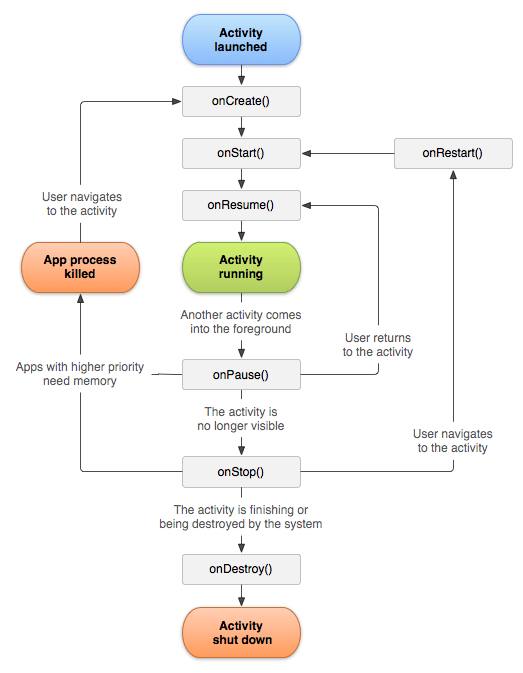
\includegraphics[width=1\linewidth]{img/cicloDeVida}
	\caption{Ciclo de vida de una \textit{Activity} en Android.}
	\label{fig:cicloDeVida}
\end{figure}

Para evitar este problema es necesario crear una forma de mantener la persistencia de los elementos. Por ello, opté por crear una base de datos en \textbf{Sqlite} como en la parte de Python. Y dentro del método \verb|onCreate| de cada ventana que lo necesite, haremos una llamada a la base de datos para obtener los elementos que teníamos antes.

En la base de datos creada para Android tenemos las tablas \textit{estancias}, \textit{elementos} y \textit{datosServidor}. Podemos observar un ejemplo de cada tabla en las tablas \ref{tabla:tablaEstancias}, \ref{tabla:tablaElementos} y \ref{tabla:tablaDatosServidor}.

\newpage
\tablaSmall{Ejemplo de datos de la tabla \textit{estancias}.}{l c c c c}{tablaEstancias}
{ \multicolumn{1}{l}{}id & nombre \\}{
	0 & Habitación 1\\
	1 & Salón 1\\
	2 & Cocina 1\\
	3 & Baño 1\\
}

\tablaSmall{Ejemplo de datos de la tabla \textit{elementos}.}{l c c c c}{tablaElementos}
{ \multicolumn{1}{l}{} estancia & nombre & estado \\}{
	Habitación 1 & Bombilla 1 & 0\\
	Habitación 1 & Bombilla 2 & 0\\
	Salón 1 & Bombilla 1 & 1\\
}

\tablaSmall{Ejemplo de datos de la tabla \textit{datosServidor}.}{l c c c c}{tablaDatosServidor}
{ \multicolumn{1}{l}{} id & ip & puerto\\}{
	0 & 192.168.X.X & 8888\\
}

\subsection{Visualización}

En este apartado visualización quiero hacer referencia a la forma de representación de las estancias y bombillas en la aplicación.

Para su correcta representación estaba buscando un método o estructura que me permitiese almacenar, modificar y eliminar de manera sencilla. Entonces se me ocurrió utilizar una \textit{ListView}, es decir, una lista de elementos. Esta estructura tiene sus propios métodos para realizar la agregación, eliminación y modificación, pero yo pretendía tener una \textit{ListView} personalizada. Pretendía que dentro de cada elemento o fila de la \textit{ListView}, se pudiese insertar más elementos como imágenes, botones, interruptores, etc. Debido a esto, no me quedó otra opción que crear una \textit{ListView} personalizada para las estancias y otra totalmente diferente para las bombillas. \\
Los elementos de la \textit{ListView} son organizados y tratados mediante un adaptador, que es el que representa los elementos en la lista. Por tanto, creé dos clases nuevas que heredasen de la clase \textit{ArrayAdapter} y así personalizarlas con mis preferencias. Una vez creadas, simplemente se crea una \textit{ListView} y se asigna un nuevo adaptador: 

\verb|listView.setAdapter(adaptador);|

Tras conseguir la estructura personalizada y que los elementos se viesen como quería, necesitaba alguna manera de que el usuario modificase los elementos de forma sencilla. Entonces se me ocurrió crear un menú contextual sobre cada elemento de la lista que permite realizar modificaciones solo sobre ese. Para conseguir que el menú contextual funcione sobre una \textit{ListView} hay que tener en cuenta que en la vista o \textit{layout} de la fila, esté activada la opción que permita mantener pulsado un largo tiempo. Es decir, necesitamos acceder a nuestro adaptador personalizado y añadir lo siguiente:

\verb|row.setLongClickable(true);|

Existe otro problema respecto a las \textit{ListView} y es que hay que tener en cuenta que los cambios realizados sobre la vista de cada elemento de la lista no van a permanecer una vez se llame a \verb|NotifyDataSetChanged()|. Este método lo que hace es cargar de nuevo los elementos de donde esta obteniendo la \textit{ListView} los datos. Por tanto, para conseguir añadir nuevos elementos y que tras llamar a este método, no desaparezcan los cambios realizados, en vez de realizar los cambios sobre la vista, tenemos que realizarlos sobre la lista desde la que toma los elementos la \textit{ListView}.

\subsection{Conexión}

Esta es la parte más importante de la aplicación Android y con la que más problemas me he encontrado.
Cuando comencé, la manera que me pareció más correcta para enviar datos al servidor era a través de un tarea asíncrona, es decir, es una ejecución independiente de la parte gráfica que estamos viendo. Dentro de ella, abría una conexión mediante un \textit{Socket}, enviaba el mensaje y lo cerraba de nuevo. 

Pronto me dí cuenta de que de esta manera yo no podría recibir mensajes del servidor en cualquier momento y me interesaba. Así que opté por hacer como en la parte del Servidor Python, crear una ejecución independiente mediante un \textbf{Thread} y escuchar siempre si llega algún mensaje del servidor.\\
Para conseguir que la ejecución de escucha del servidor funcionase tuve que crear una nueva clase que implementase la interfaz \textit{Runnable} y de está manera meter mi código en el método \verb|run()|. Además, una ventaja que tiene ser una ejecución independiente, es que no se interrumpe a pesar de realizar cambios entre ventanas. Yo quería que el mensaje que llegase fuese mostrado en pantalla y no es posible mostrar un mensaje en pantalla desde una ejecución independiente que no tiene parte gráfica.\\
Estuve indagando sobre como poder mandar mensajes, incluso objetos, desde un \textbf{Thread} a la parte gráfica y me encontré con la clase \textit{Handler} \cite{android:Handler}. La clase \textit{Handler} permite enviar y procesar mensajes y objetos asociados a la cola de un hilo. Entonces me di cuenta de que la manera de poder transportar el dato \textit{String} obtenido del servidor es encapsulado a través de un objeto \textit{Bundle}.

El método \verb|sendMessage| nos permite poner en la cola un objeto \textit{Message} que contendrá nuestro \textit{Bundle} con nuestros \textit{String} recibido. Una vez nuestro \textit{Bundle} llegue, será procesado por el método \verb|handleMessage|. Entonces lo ideal es sobreescribir ese método en una de las \textit{Activity} para poder realizar los cambios pertinentes sobre el dato recibido.

A la hora de la creación del \textit{Socket}, es mejor optar por crear un \textit{Socket} sin conexión mediante el constructor vacío y luego conectarlo, que intentar instanciar un \textit{Socket} con una ip y un puerto al inicio.\\
Otro problema respecto a la escucha del servidor es que cada vez que se trataba de conectar a través de la ventana del Servidor se creaba un nuevo hilo y esto daba lugar a que pudiésemos tener más de 5 hilos activos a la vez. Para solucionar este problema traté de usar un patrón de diseño \textit{Singleton}, que haría que solamente hubiese una única conexión y fuese accesible desde cualquier punto de la aplicación. De esta manera podemos realizar la conexión al servidor según entremos a la aplicación desde la ventana principal.
No he seguido el patrón de diseño al pie de la letra ya que en él se especifica que el objeto no tiene parámetros, pero el mío si los tiene. Y esto sucede porque a la hora de implementar la posibilidad de ser más usuarios conectados al servidor, necesitaba una manera de saber en que ventana nos encontramos para actualizar sus elementos según el mensaje que llegue.\\
Además este patrón de diseño ha sido usado debido a que para cerrar la conexión activa con el servidor, necesitamos acceder a la instancia de \textit{RecepcionSocket} que se usó para la creación del hilo. Es decir, de está manera, la conexión que se crea en la ventana principal es posible cerrarla desde la ventana del Servidor, ya que estamos accediendo a la misma instancia \textit{RecepcionSocket} que se usó en la creación.

Por último, quería decir que he tenido muchos problemas a la hora de saber si la conexión ha llegado a conectarse, está activa o cerrada. Es decir, si yo quisiese saber si ahora mismo estamos conectados al servidor, no he encontrado una manera sencilla de averiguarlo. El problema es que los métodos de los que nos provee la clase \textit{Socket} no son nada claros.

\begin{itemize}
	\item El método \verb|isConnected()| \cite{android:isConnected} de la clase \textit{Socket} indica que cerrar un \textit{socket} no borra su estado de conexión, lo que significa que este método devolverá un \textbf{True} aunque el \textit{socket} esté cerrado si se ha llegado a conectar alguna vez.
	\item El método \verb|close()| \cite{android:close} de la clase \textit{Socket} indica que una vez se ha cerrado el \textit{socket} no estará disponible para nuevas conexiones, es decir, no puede ser reconectado. Por tanto, es necesario crear una nueva instancia del \textit{Socket}.
\end{itemize}

Esto hace que haya muchos problemas para saber si tenemos una conexión activa con el servidor.

\capitulo{6}{Trabajos relacionados}

En este apartado voy a hablar sobre un proyecto parecido a este, pero que está actualmente funcionando. \\
La empresa Xiaomi tiene actualmente una aplicación como la mía en la tienda \textit{Google Play}, desde la cuál se pueden sincronizar los dispositivos Xiaomi que lo permitan y cambiar parámetros de ellos.

Actualmente, poseo una bombilla de esta marca como la de la imagen \ref{fig:yeelight} y cuenta con muchas posibilidades, entre ellas modificar su estado, color, intensidad y modo desde la propia aplicación de Xiaomi. Lo único que se necesita para que funcione es que el interruptor de la corriente esté encendido y que el dispositivo esté sincronizado con la aplicación.\\

\begin{figure}[h!]
	\centering
	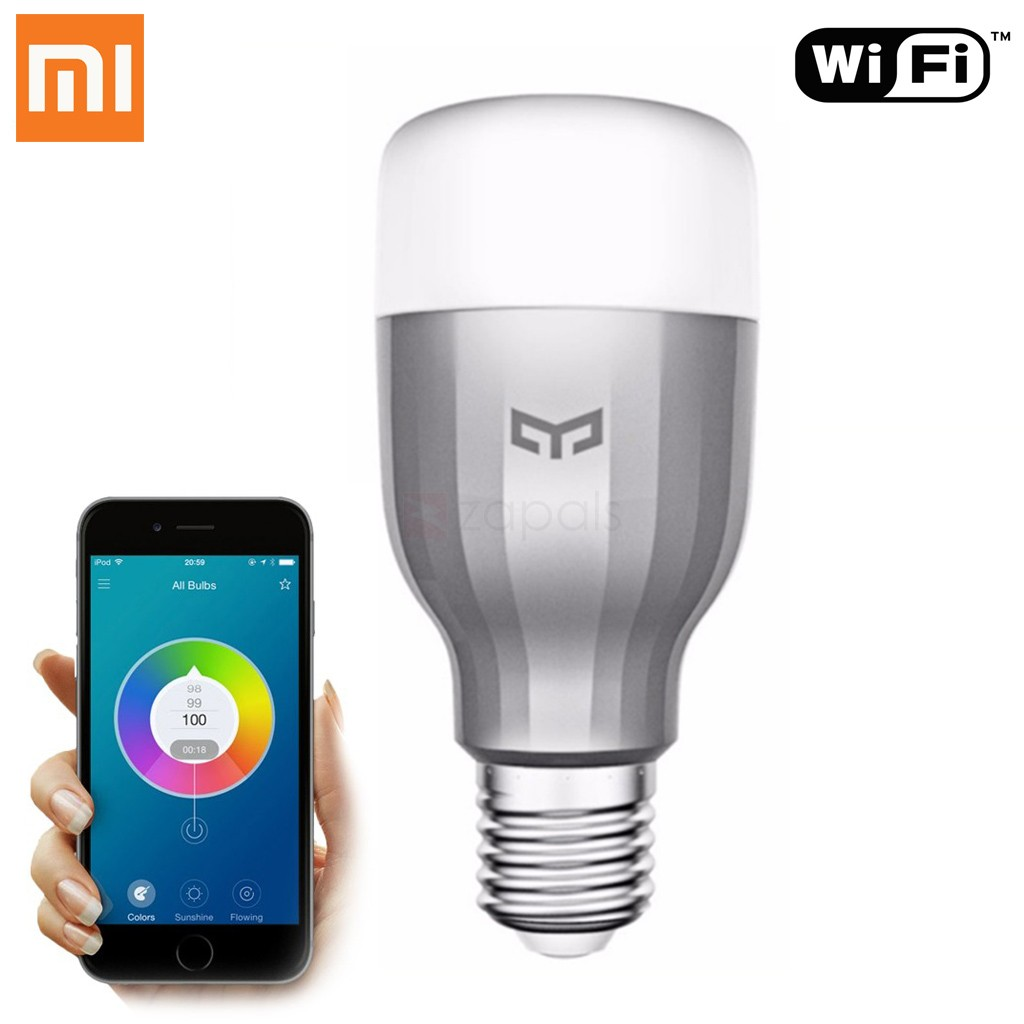
\includegraphics[width=0.35\linewidth]{img/xiaomiYeelight}
	\caption{Bombilla inteligente de la marca Xiaomi.}
	\label{fig:yeelight}
\end{figure}

La aplicación \textit{Mi Home} de Xiaomi se puede encontrar en \textit{Google Play} en el siguiente enlace \url{https://play.google.com/store/apps/details?id=com.xiaomi.smarthome&hl=es}.
\capitulo{7}{Conclusiones y Líneas de trabajo futuras}

Todo proyecto debe incluir las conclusiones que se derivan de su desarrollo. Éstas pueden ser de diferente índole, dependiendo de la tipología del proyecto, pero normalmente van a estar presentes un conjunto de conclusiones relacionadas con los resultados del proyecto y un conjunto de conclusiones técnicas. 
Además, resulta muy útil realizar un informe crítico indicando cómo se puede mejorar el proyecto, o cómo se puede continuar trabajando en la línea del proyecto realizado. 



\bibliographystyle{plain}
\bibliography{bibliografia}

\end{document}
